\section{Resolución de corto}
\begin{enumerate}
    \item Que cualidad tiene un bien inmediato.
    \item Bienes superiores e inferiores.
    \item Cuando un bien inmediato pierde su valor.
\end{enumerate}

%%%%%%%%%%%%%%%%%%%%%%%%%%%%%%%%%%%%%%%%%%%%%%%%%%%%%%%%%%%%%%%%%%%%%%%%%%%%%%%%%%%%%%%%%%%%%%%%
\section{Noticia}
\begin{itemize}
    \item ¿Quién tiene el poder de crear dinero en la economía moderna?
    \item El dinero viene de Bancos privados, dinero no tangible\dots.
    \item El dinero se genera por medio de préstamos bancarios.
    \item Dinero físico y dinero electrónico (25-1).
    \item \textbf{Nos preguntamos:} ¿el banco crea dinero? por medio de préstamos te dan dinero que no existía antes.
    \item El banco central, políticas monetarias.
    \item Peligros en el aumento en la desigualdad de ingresos, se tiende a prestarle a los que ya tienen y no a los que no.
\end{itemize}

\section{Análisis }
\begin{itemize}
    \item Los límites del banco:
    \begin{itemize}
        \item \textbf{El interno}: estimación si me van a poder devolver el préstamos. En cierta manera el banco se endeuda conmigo, el pago \textbf{compra mi pagaré}, sigue siendo un pagaré y cuando se incumple los bancos quiebran; \emph{Citación:``si todos vamos al banco a la vez nuestro dinero no va a estar ahí, ahí es cuando interfiere el banco central para salvar el banco"}. \newline 
        \emph{\textbf{Definición de ``Coheficiente de reserva":} dado la siguiente fórmula }
        \[
          C.R. = \frac{\text{Reservas}}{\text{Depósito}} 
        \]
        Usualmente es legalmente de 16\%
        \begin{center}
            \begin{tabular}{ | p{5cm} | p{5cm} | }
            \hline
            \multicolumn{2}{|c|}{Banco}\\
            \hline
            Reservas (Q) &  Depósito \\ 
            + Préstamos & Depósito \\ 
            & Si el banco sigue dando depósitos como bestia los depósitos son demaciados. \\ 
            \hline
            \end{tabular}
        \end{center} 
        
        \begin{itemize}
            \item \textbf{\emph{(Ejemplo: La ley de no hablar mal del banco, ley de pánico financiero)}}.
            \item Cuando se usa una targeta de crédito se transfiere lo que el banco te iba a depositar (pagaré) a el establecimiento. 
        \end{itemize}
        
        \item El \textbf{límite externo} es la liquidez legal.
    \end{itemize}
\end{itemize}


El problema el proceso productivo esta dado por la siguiente línea:

\begin{center}
\begin{tabular}{ | p{5cm}  p{5cm} |  }
    \multicolumn{2}{|c|}{t=0 ----------------------------------------------t=1}   \\ 
    Inversión (orden superior)&  Bien del primer orden \\ 
    Estos bienes tienen valor por que en el futuro puede producir bienes de primer orden & este precio es una especulación\\ 
    \multicolumn{2}{|c|}{Alternativamente} \\ 
    \\
    \multicolumn{2}{|c|}{t=-1 ----------------------------------------------t=0} \\ 
    Inversión (Bien Superior) & Bien de primer orden \\ 
\end{tabular}
\end{center}

\begin{itemize}
    \item La mayor cantidad de precios están en los bienes de primer orden.
    \item Robinson Crusoe: 
    \begin{itemize}
        \item Tiene que procurarse los bienes para su supervivencia.
        \item \textbf{Nos preguntamos:} ¿Cómo hace esto? Cazando, etcétera.
        \item Pero \textbf{empieza a ahorrar} ¿cómo ahorra? acumulando comida por Ejemplo
        \item \textbf{Nos preguntamos:} ¿por qué ahorra?
        \begin{itemize}
            \item Para reducir incertidumbre
            \item Para \textbf{inversión} en términos de hacer otras cosas con el tiempo.
            \item Sin ahorro no hay inversión.
            \item Por ejemplo ahorra para tomar unos días de descanso, o tomarse el día para fabricar un instrumento capaz de ahorrarle trabajo.
            \item La creacion de producción, inversión en creación de bienes de orden superior y la creación de métodos indirectos de producción.  %AUDIO 45:10
            \item El ahorro puede permitir que después de alguna cantidad de ahorro puede designar un tiempo para la construcción de otros bienes.
        \end{itemize}
        
        \item ¿Las economías capitalistas son consumistas? Son más productivas, más aun que lo es consumista. Se ve más consumo pero le dedican más renta a el no consumo, es decir a los bienes de orden superior.
        \item Los países pobres tienden hacer más consumistas.
        \item \textbf{Nos preguntamos:} ¿Se puede ejercer la función empresarial en una economía de una persona? \textbf{Nos preguntamos:} ¿Se puede tomar el papel una persona de la persona A,B y C pagar e invertir?
    \end{itemize}
\end{itemize}


\subsection{Renta física \& Renta Económico}
\begin{tabular}{ | p{5cm} | p{5cm} |}
    \hline
    La renta física & Los bienes de orden superior determinan el costo de los bienes de ordenes de inferior, va hacia abajo  \\ 
    \hline
    La renta económica & Los bienes de orden inferior determinan el costo de los bienes de orden superior \textbf{esta es la correcta}, el precio de los bienes de orden inferiores determinan el valor de  los bienes de orden superior. Va subiendo.\\ 
    \hline
\end{tabular}



\begin{itemize}
    \item La renta física es la incorrecta, bajo esta premisa ninguna empresa podría quebrar.
    \item La renta económica toma en cuenta la teoría de valor subjetivo. \textbf{el mercado expulsa a aquellos que no saben usar bienes superiores}.
    \item No es verdad que los ricos son cada vez más ricos y los pobres cada vez más pobres.
\end{itemize}


\begin{figure}[htbp]
    \centering
    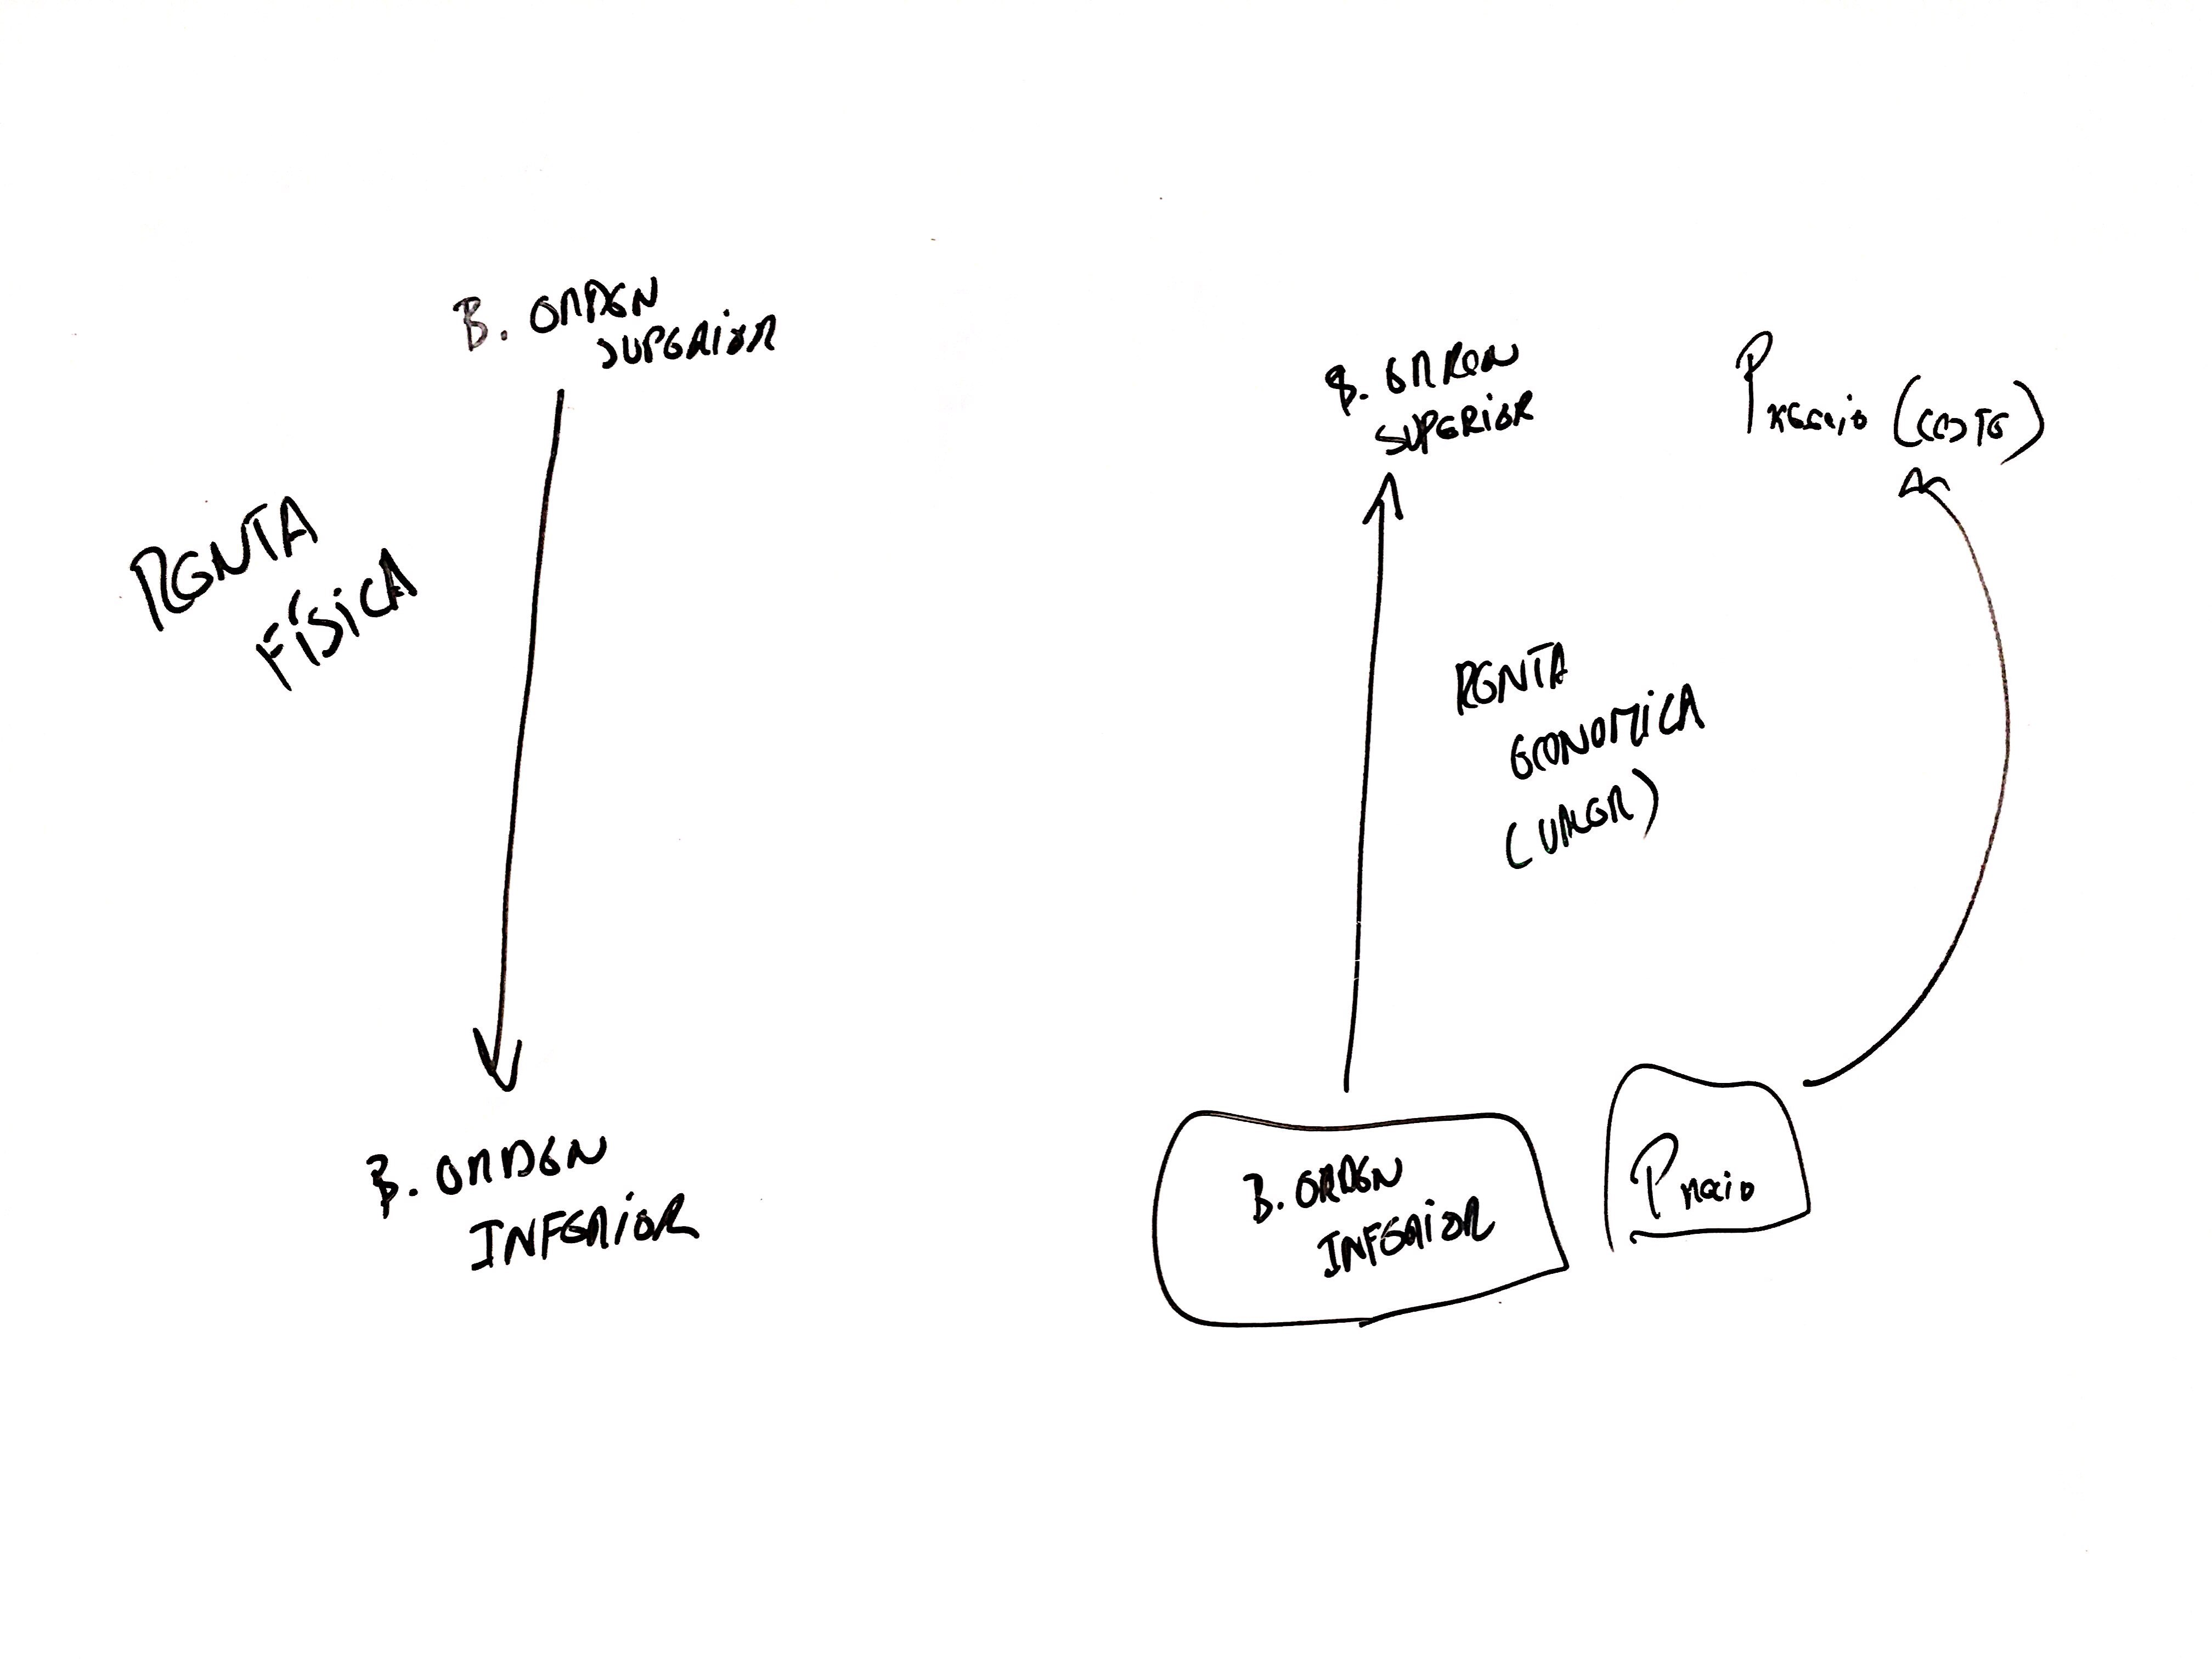
\includegraphics[width=10cm]{Classes/Images/2019-09-02-01.jpg}
    \caption{Renta física y renta económica}
    \label{}
\end{figure} 
